To be able to calculate rate constants, we need to have an accurate measure of the absolute pressure of the gas of interest. This is easier said than done, various instruments may have different absolute readings and uncertainties and may not agree with one another in situ. To find the relative pressures of multiple gasses introduced into the chamber, we use the RGA, but Stanford Research Systems does not provide an uncertainty for its device's absolute accuracy. We calibrate it by cross-correlating our RGA measurements with the total pressure measured by an Agilent UHV-24 Bayard-Alpert Gauge Tube, which gives a quoted $<10\%$ error at $5 \times 10^{-10}$ Torr (our normal operating pressure). The fact that the ion gauge is set in a nipple connected to the chamber provides at least another 30\% uncertainty, but is more acceptable than the completely unknown reliability of the RGA.

The calibration consists of incrementally adding either \ce{H2} or \ce{H2O} into the chamber and read off the pressures from the RGA as well as the ion gauge (scaled by their species dependent specifications). By fitting the relationship between these two readings, we find that there is a mass dependent scaling factor for the RGA to ion gauge pressure shown in Figure \ref{fig: rga calibration}. \ce{H2O} is scaled by 1.1, while \ce{H2} is much less accurate, and scaled by 0.59. Using this calibrated pressure reading, our measured \ce{Be+ + H2} reaction rate coefficient of $1.2 \pm 0.3_{\text{stat}} \times 10^{-9}$ cm$^3$/s) agrees with the literature seen in Figure \ref{fig: Be+H2 calibration}.

\begin{figure}[H]
	\centering
	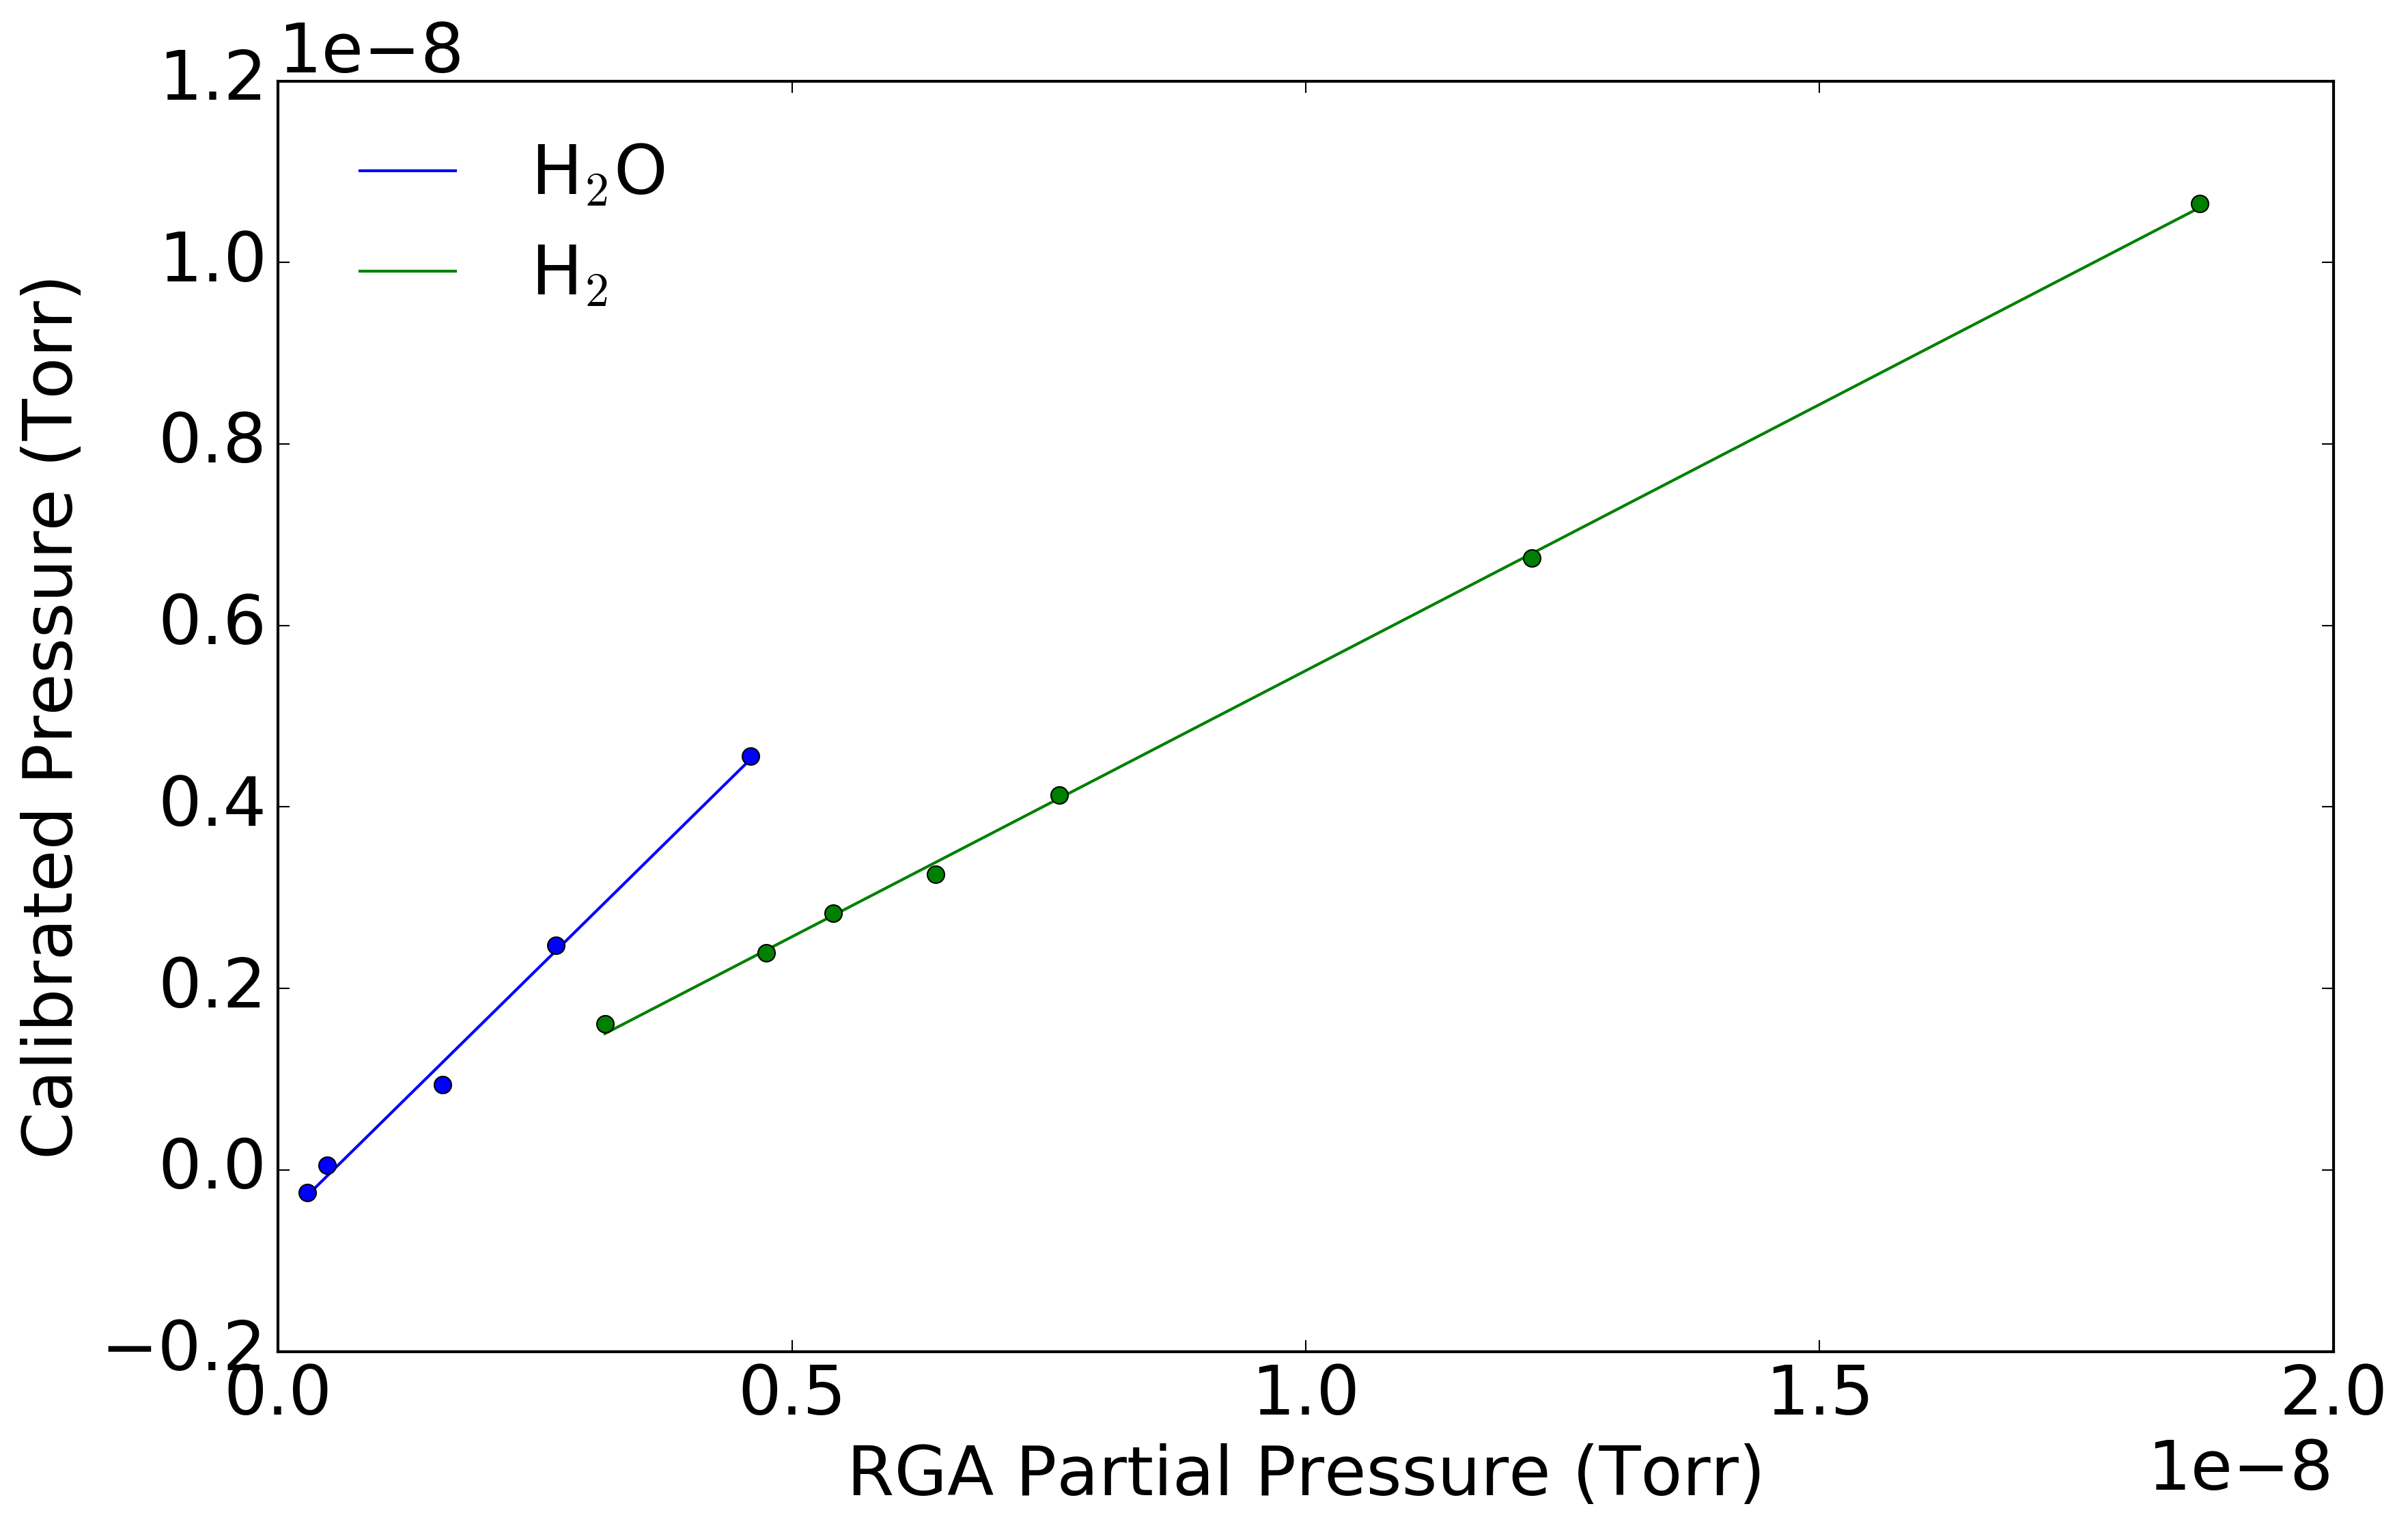
\includegraphics[width=0.8\textwidth]{images/pressure_calibration.png}
	\caption{Fitted curves for \ce{H2} and \ce{H2O} detection between the ion gauge and RGA. The reported pressure between the ion gauge and RGA is nearly identical for \ce{H2O} with a slope of 1.1, but noticeably different for \ce{H2} with a slope of 0.59.}
	\label{fig: rga calibration}
\end{figure}

\begin{figure}[H]
	\centering
	\begin{tabular}{cc}
		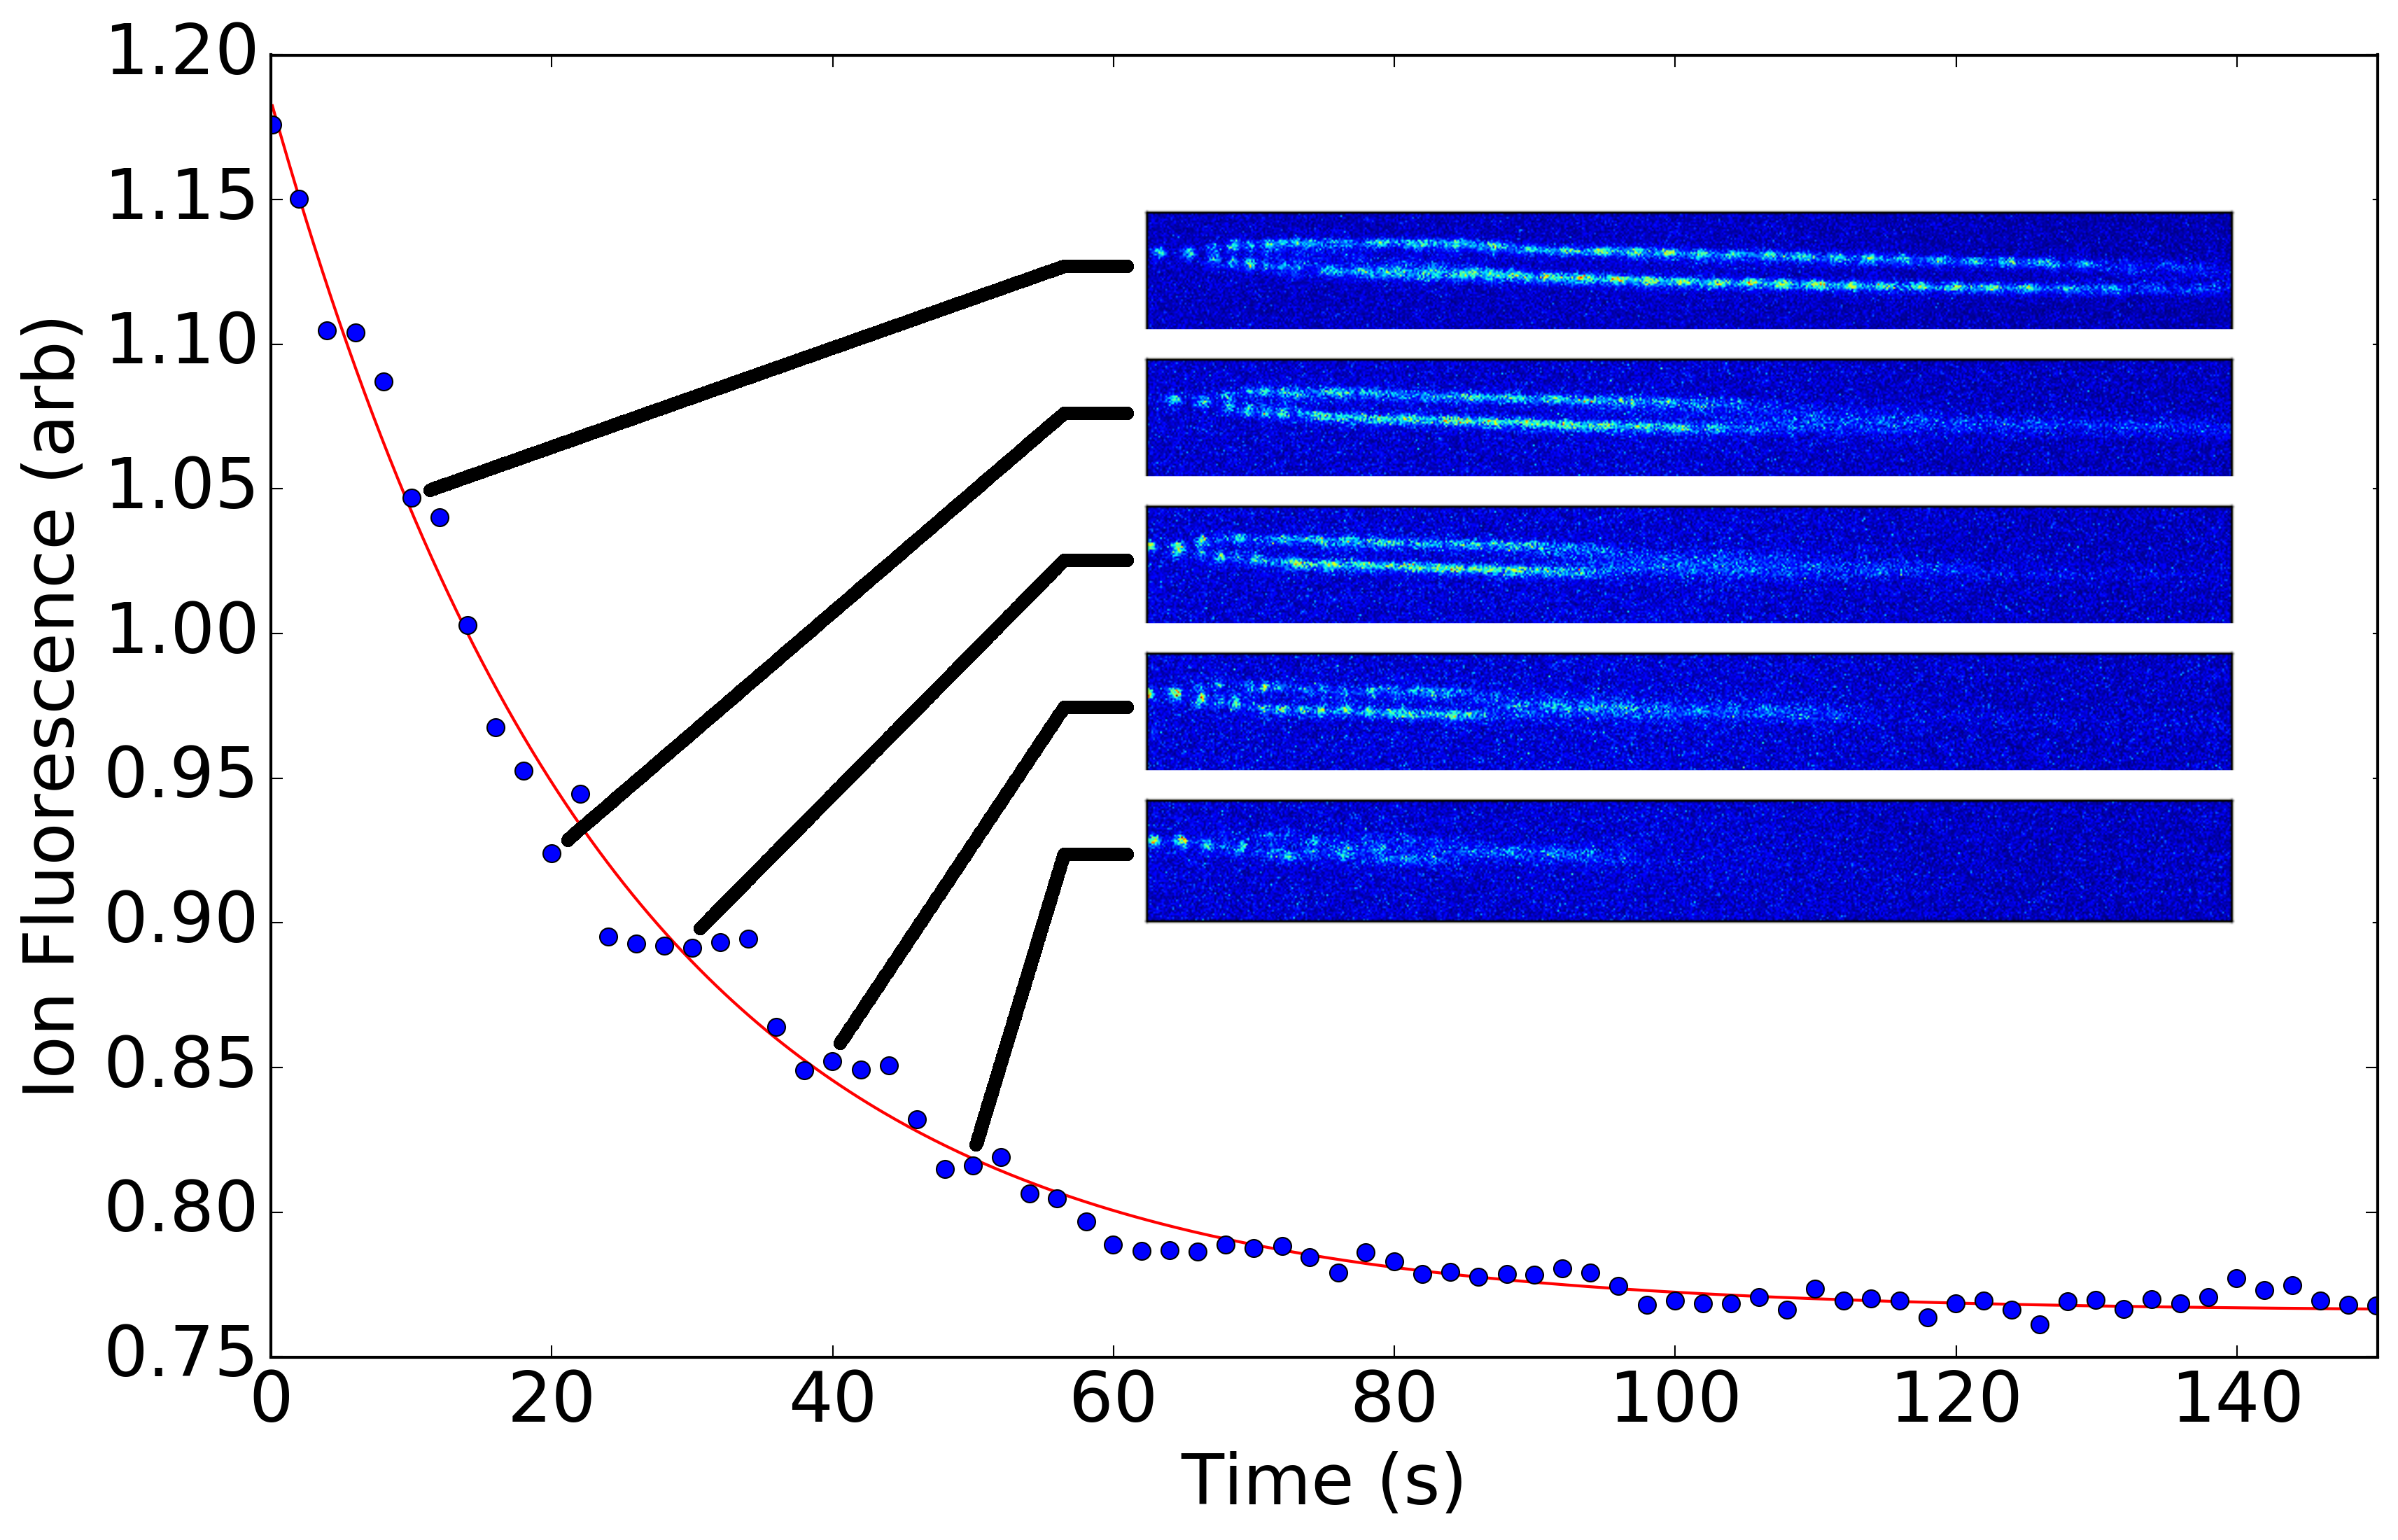
\includegraphics[width=0.5\textwidth]{images/Be_H2_decay_images.png} &
		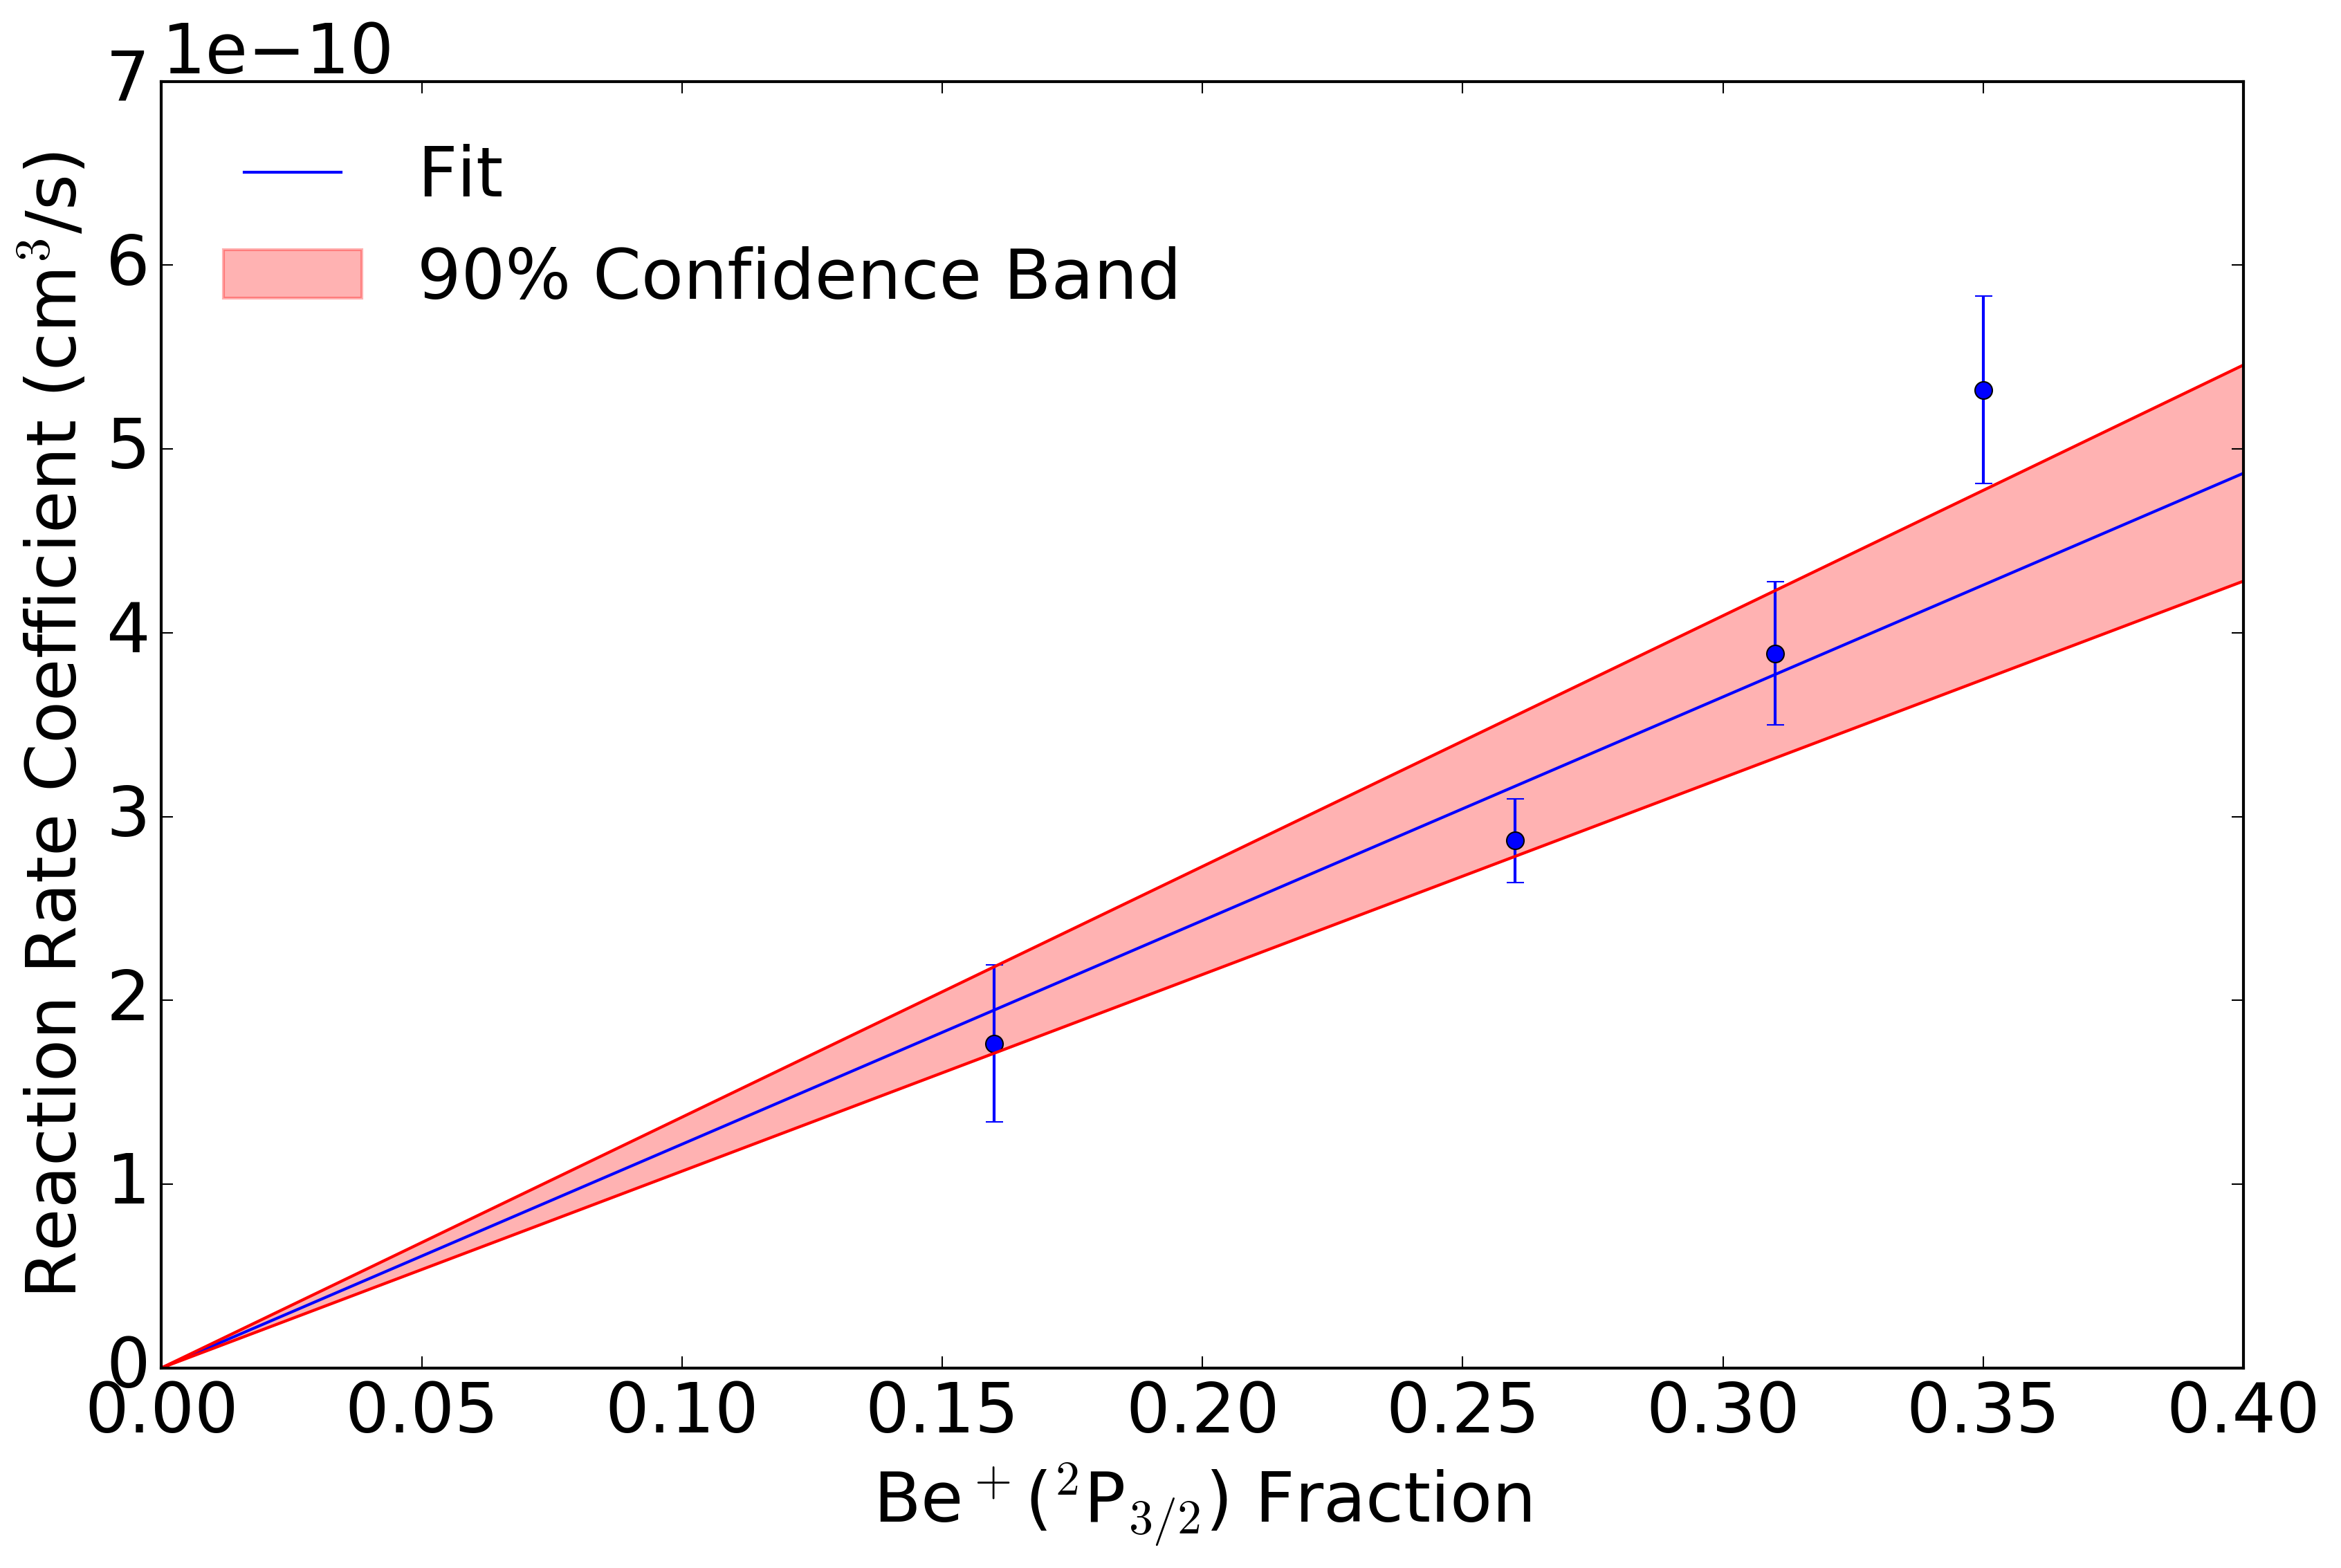
\includegraphics[width=0.5\textwidth]{images/Be_H2_fit.png}
	\end{tabular}
	\caption{(A) A typical fluorescence decay measurement of \ce{Be+ + H2}. The inset images are a subset of the original ion fluorescence images recorded by the camera. The red curve is an exponential fit (with a free offset) to the data, which gives the total reaction rate. (B) A fit of \ce{Be+ + H2} fluorescence decay at various P state excitation fractions. A statistical rate coefficient for full excitation of $(1.2 \pm 0.3_{\text{state}}) \times 10^{-9}$ cm$^3$/s is in agreement with existing literature.}
	\label{fig: Be+H2 calibration}
\end{figure}